\documentclass[a4paper, 11pt]{article}

\usepackage[left=1.5cm, right=1.5cm, top=2cm, bottom=2cm]{geometry}

\usepackage[utf8]{inputenc} 
\usepackage[T1]{fontenc}      
\usepackage[french,english]{babel}  
\usepackage{lmodern}

\usepackage{amsmath, mathtools}
\usepackage{amssymb}
\usepackage{amsthm}
\usepackage{empheq}

\usepackage{graphicx,wrapfig}
\usepackage{subfig}

\usepackage{listings}
\usepackage{color} %red, green, blue, yellow, cyan, magenta, black, white
\definecolor{mygreen}{RGB}{28,172,0} % color values Red, Green, Blue
\definecolor{mylilas}{RGB}{170,55,241}

\graphicspath{{../figures/}}
\usepackage{caption}

\begin{document}
\title{Rendu DM2 Modèles probabilistes graphiques} 
\author{Yoann Pradat}
\maketitle

\paragraph{Exercise 1}

1.1 A probability distribution $p$ is in $\mathcal{L}(G)$ if it satisfies

\begin{equation}
  \forall x,y,z,t \quad p(x,y,z,t) = p(x)p(y)p(z|x,y)p(t|z) 
\end{equation}

It is not true to say that $X \bot Y | T$. As a proof, let's imagine a family where $X = $ nb of girls, $Y = $ nb of
boys, $Z =$ nb of blue-eyed children and $T =$ nb of marriages. We suppose that only blue-eyed children can get married 
with probability $\frac{1}{2}$. Let $p$ be the joint distribution of these 4 variables. Using definition of conditional 
probability we have $p(x,y,z,t) = p(x) p(y|x) p(z|x,y) p(t|x,y,z)$. X and Y are clearly independent so $p(y|x) = p(y)$.
Knowing X and Y is redundant to knowing Z for the variable T, therefore $p(t|x,y,z) = p(t|z)$. Consequently $p \in
\mathcal{L}(G)$. However, it is clearly wrong to say that $p(x|y,t) = p(x|t)$ as knowing for example that $y=0$ and that 
$t >0$ gives more information on $x$ that simply $t>0$. In the first case there must be at least $t$ girls, in the second
case the number of girls may be anything.

\clearpage

\paragraph{Exercise 2}

\textbf{2.1} Let's show that $\mathcal{L}(G) = \mathcal{L}(G')$. We know that

\begin{equation}
  p \in \mathcal{L}(G) \iff p(x) = \prod_{i=1}^n p(x_i|x_{\pi_i}) \quad \text{and} \quad  p \in \mathcal{L}(G') \iff
  p(x) = \prod_{i=1}^n p(x_i|x_{\pi'_i}) 
\end{equation}

Flipping the edge $\{i \to j\}$ to $\{j \to i\}$ only affects the parents of $i$ and $j$. Therefore, for any $l$
different from $i$ and $j$, $\pi'_l = \pi_l$. It remains to prove that $p(x_i|x_{\pi_i}) p(x_j|x_{\pi_j}) = 
p(x_i|x_{\pi'_i}) p(x_j|x_{\pi'_j})$. \\

First we note that $\pi'_i = \pi_i \cup \{j\}$ and $\pi'_j = \pi_j \backslash \{i\} = \pi_i$. Therefore what we want to prove is
$p(x_i|x_{\pi_i}) p(x_j|x_{\pi_j}) = p(x_i|x_{\pi_i}, x_j) p(x_j|x_{\pi_i})$. Simply using definition of conditional
probability we have

\begin{align*}
  p(x_i|x_{\pi_i}, x_i) &= \frac{p(x_j, x_{\pi_i}, x_i)}{p(x_{\pi_i}, x_i)} \\
  &= \frac{p(x_i|x_{\pi_i}, x_j)p(x_{\pi_i}, x_j)}{p(x_{\pi_i}, x_i)}.
\end{align*}

Putting the denominator on the left side and dividing both sides by $p(x_{\pi_i})$ gives the result we want. Therefore,

\begin{equation}
p \in \mathcal{L}(G) \iff p \in \mathcal{L}(G') 
\end{equation}

\textbf{2.2} Given that G is a directed tree, each node has exactly one parent except for the root that has no parent
and that we will denote $x_1$. Therefore $p \in \mathcal{L}(G) \iff p(x) = p(x_1)p(x_2|x_{\pi_2})\dots
p(x_n|x_{\pi_n})$ and $p \in \mathcal{L}(G') \iff p(x) =
\psi_1(x_1)\dots\psi_n(x_n)\psi_{2,\pi_2}(x_2,x_{\pi_2})\dots\psi_{n,\pi_n}(x_n,x_{\pi_n})$ where $x_j$ is a
parent of $x_i$ in $G'$ $x_j$ was a parent of $x_i$ in the directed tree $G$. \underline{Rk}: The normalizing constraint 
is hidden in the $\psi$ functions (as if I had defined new $\psi$ functions).\\

Clearly $p \in \mathcal{L}(G) \implies p \in \mathcal{L}(G')$. One can choose for instance $\psi_1(x_1) = p(x_1)$, $\psi_i
\equiv 1$ for $i \geq 2$ and $\psi_{i, \pi_i}(x_i, x_{\pi_i}) = p(x_i|x_{\pi_i})$.\\

Now suppose $p \in \mathcal{L}(G')$. Let's define 

\begin{align*}
\phi_i(x_i) &= \sum_{x_{V\backslash \{i\}}} \prod_{l \in V\backslash \{i\}} \psi_l(x_l) \prod_l \psi_{l, \pi_l}(x_l, x_{\pi_l}) \\
\phi_{i,\pi_i}(x_i, x_{\pi_i}) &= \sum_{x_{V\backslash \{i, \pi_i\}}} \prod_{l \in V\backslash \{i, \pi_i\}} \psi_l(x_l) 
\prod_{l \in V\backslash \{i\}} \psi_{l, \pi_l}(x_l, x_{\pi_l})
\end{align*}

Then $p(x_i) = \psi_i(x_i) \phi_i(x_i)$ and $p(x_i, x_{\pi_i}) = \psi_i (x_i) \psi_{\pi_i} (x_{\pi_i}) \psi_{i,\pi_i}(x_i,x_{\pi_i}) 
\phi_{i, \pi_i}(x_i, x_{\pi_i})$. As a consequence

\begin{align*}
  p(x_1) p(x_2|x_{\pi_2}) \dots p(x_n|x_{\pi_n}) &= \psi_1(x_1) \phi_1(x_1) \frac{\psi_2(x_2)\psi_{2, \pi_2}(x_2,
  x_{\pi_2}) \phi_{2, \pi_2}(x_2, x_{\pi_2})}{\phi_{\pi_2}(x_{\pi_2})} \dots 
  \frac{\psi_n(x_n)\psi_{n, \pi_n}(x_n, x_{\pi_n}) \phi_{n, \pi_n}(x_n, x_{\pi_n})}{\phi_{\pi_n}(x_{\pi_n})} \\ 
  &= p(x) \frac{\phi_1(x_1) \prod_{l=2}^n \phi_{l, \pi_l}(x_l, x_{\pi_l})}{\prod_{l=2}^n \phi_{\pi_l}(x_{\pi_l})}
\end{align*}

Noting that $\phi_{\pi_i}(x_{\pi_i}) = \sum_{x_i} \phi_{i, \pi_i}(x_i, x_{\pi_i}) \psi_i(x_i) \psi_{i, \pi_i}(x_i,
x_{\pi_i})$ and that each node has only one parent is is not too hard to show that the fraction is one. \\

Therefore $p \in \mathcal{L}(G)$.

\clearpage

\paragraph{Exercise 3}

\textbf{3.1} In the figure~\ref{fig:kmeans} on the next page,
I ran k-means for distances of order 1 and 2, each for 3 different seeds. We see that different initializations give
slightly different clusters and that the shape of the cluster depends on the distance used. Usually when we do such
clustering, we run several initialization and keep the one with the lowest total distance.\\

\textbf{3.2} Let $Z \in \{1, \dots, k\}$ ($k=4$ here) be the latent variable, $X$ be the d-dimensional observations. Let $\pi = (\pi_1,
\dots, \pi_k)$ be the parameters of $Z$. We suppose $X|Z=j$ is normally distributed with parameters $\mu_j, \Sigma_j$.
We saw in class the form of the complete log-likelihood

\begin{equation}
\log p_{\theta}(x,z) = \sum_{i=1}^n \log p_{\theta}(x_i,z_i) = \sum_{i=1}^n \sum_{j=1}^k z_i^j \log(\pi_j) +
\sum_{i=1}^n \sum_{j=1}^k z_i^j \log \mathcal{N}(x_i|\mu_j, \Sigma_j)
\end{equation}

The E-step consists in taking the expectation of this log-likehood with respect to the conditional distribution of Z
given X. This is done by simply replacing $z_i^j$ with $\tau_i^j = \frac{\pi_j \text{det}(\Sigma_j)^{\frac{-1}{2}}
e^{-\frac{1}{2}(x_i-\mu_j)^t \Sigma_j^{-1} (x_i-\mu_j)}}{\sum_{l=1}^k \pi_l \text{det}(\Sigma_l)^{\frac{-1}{2}} 
e^{-\frac{1}{2}(x_i-\mu_l)^t \Sigma_l^{-1} (x_i-\mu_l)}}$. 

The M-step consists in maximizing the expected value of the complete likelihood with respect to $\theta=(\pi, \mu,
\Sigma)$. To MLE of $\pi$ is simply obtained by maximizing $\sum_{i=1}^n \sum_{j=1}^k \tau_i^j \log(\pi_j)$ with
constraint $\sum_{j=1}^k \pi_j = 1$. Equalizing partial derivatives of the Lagrangian to 0 gives the formula.
The MLE estimate of $\mu_j$ is obtained by maximizing $\sum_{i=1}^n \sum_{j=1}^k -\frac{1}{2} \tau_i^j (x_i-\mu_j)^t 
\Sigma_j^{-1} (x_i-\mu_j)$. Again, equalizing partial derivatives to 0 gives the estimators.

\begin{equation}
 \boxed{\forall j \in \{1, \dots, 4\} \quad \widehat{\pi_j} = \frac{\sum_{i=1}^n \tau_i^j}{\sum_{i=1}^n \sum_{l=1}^k \tau_i^l}  \qquad \widehat{\mu_j} =
 \frac{\sum_{i=1}^n \tau_i^j x_i}{\sum_{i=1}^n \tau_i^j}}
\end{equation}

We suppose covariance matrices proportional to identity i.e $\Sigma_j = \sigma_j^2 I$. Then the MLE estimate $\sigma_j^2$ is
obtained by maximizing $\sum_{i=1}^n \sum_{j=1}^k \tau_i^j (-\frac{d}{2} \log(\sigma_j^2) - \frac{1}{2\sigma_j^2}(x_i -
\mu_j)^t (x_i - \mu_j))$. On en déduit 

\begin{equation}
 \boxed{ \forall j \in \{1, \dots, 4\} \quad \widehat{\sigma_j^2} = \frac{\sum_{i=1}^n \tau_i^j (x_i - \mu_j)^t (x_i -
 \mu_j)}{d\sum_{i=1}^n \tau_i^j}}
\end{equation}

\textbf{3.3} We don't suppose anymore that $\Sigma_j = \sigma_j^2 Id$. The MLE for all the other parameters than $\Sigma_j$ stay
the same. Regarding $\Sigma_j$, we now have to maximize  $\sum_{i=1}^n \sum_{j=1}^k \tau_i^j (-\frac{1}{2}
\log(\text{det }\Sigma_j) - \frac{1}{2}(x_i - \mu_j)^t \Sigma_j^{-1} (x_i - \mu_j))$. Using the fact that the gradient
with respect to $Q$ of $\log(\text{det } Q)$ is $Q^{-1}$ and the trace trick for the second term to compute the
gradient, we find MLE estimator of $\Sigma_j$

\begin{equation}
 \boxed{ \forall j \in \{1, \dots, 4\} \quad \widehat{\Sigma_j} = \frac{\sum_{i=1}^n \tau_i^j (x_i - \mu_j)(x_i -
 \mu_j)^t}{\sum_{i=1}^n \tau_i^j}}
\end{equation}

\textbf{3.4} The gaussian mixture model with full covariance matrix gives a better fit that the gaussian mixture
model with covariances proportional to identity. It is quite clear from the data that for 2 of the 4 distributions
assumed the variances in each direction are very different. IdGMM has a log-likelihood of -2,689.34 on the train set,
-2,665.30 on the test set where as it is respectively -2,345.97, -2,425.99 for the model FullGMM. This is confirms 
our observation that the full model is a better fit.

\clearpage

\begin{figure}[!h]
  \centering
  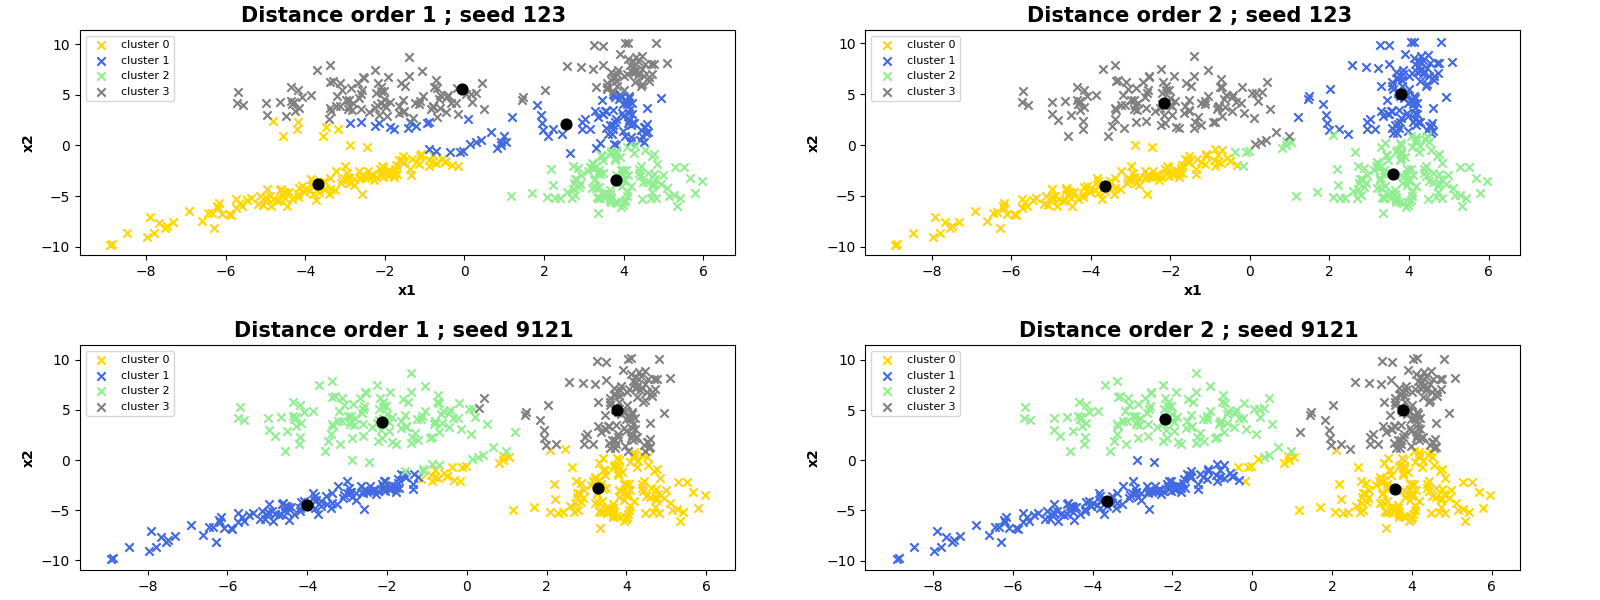
\includegraphics[width=18cm]{kmeans.png}
  \caption{Examples KMeans algorithm on train data}
  \label{fig:kmeans}
\end{figure}

\begin{figure}[!h]
  \centering
  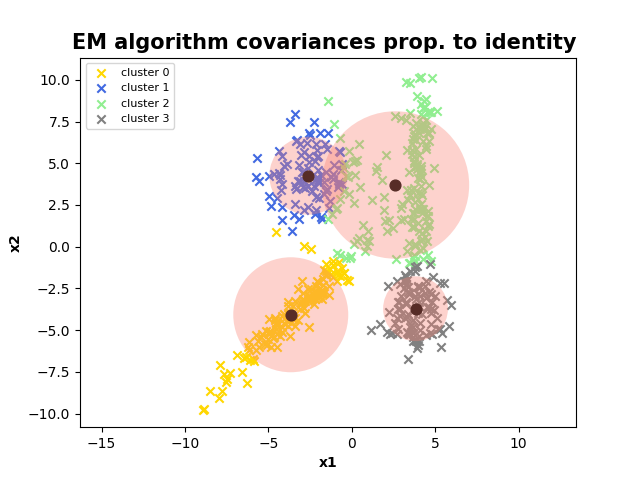
\includegraphics[width=9cm]{em_iso.png}
  \caption{Isotropic covariance EM algorithm on train data}
  \label{fig:em_iso}
\end{figure}

\begin{figure}[!h]
  \centering
  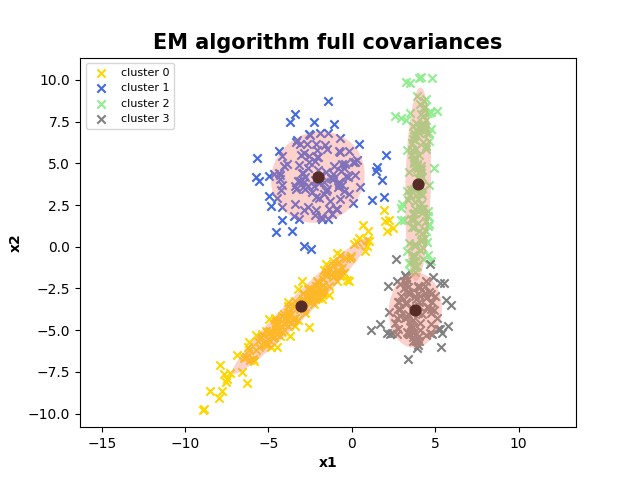
\includegraphics[width=9cm]{em_full.png}
  \caption{Full covariance EM algorithm on train data}
  \label{fig:em_full}
\end{figure}

\end{document}



